\documentclass{beamer}

\mode<presentation>
{
    \usetheme{default}
    \usecolortheme{default}
    \usefonttheme{default}
    \setbeamertemplate{navigation symbols}{}
    \setbeamertemplate{caption}[numbered]
}

\usepackage[english]{babel}
\usepackage[utf8]{inputenc}
\usepackage[T1]{fontenc}
\usepackage{graphicx}
\usepackage{hyperref}

\title[Project Presentation]{Project Presentation}
\author{Alessandro Lombardi}
\institute{Artificial Intelligence - University of Bologna}
\date{08-05-2020}

\begin{document}

    \begin{frame}
        \titlepage
    \end{frame}

    \begin{frame}{Outline}
        \tableofcontents
    \end{frame}

    \section{Introduction}\label{sec:introduction}

    \begin{frame}{Introduction}
        \begin{block}{The idea}
            Analyze Ethereum Blockchain as a network of transactions between addresses.
        \end{block}

        \vskip 1cm

        \begin{block}{The Ethereum Blockchain}
            Some stats to get an idea of the involved numbers
            \begin{itemize}
                \item latest \textbf{block} height value higher than 10 million
                \item more than 96 million unique \textbf{addresses}
                \item more than 698 million \textbf{transactions}
                \item Ethereum blocks are mined every 20 seconds
            \end{itemize}
            Source: \url{https://etherscan.io/}
        \end{block}

    \end{frame}

    \begin{frame}{}
        \begin{figure}
            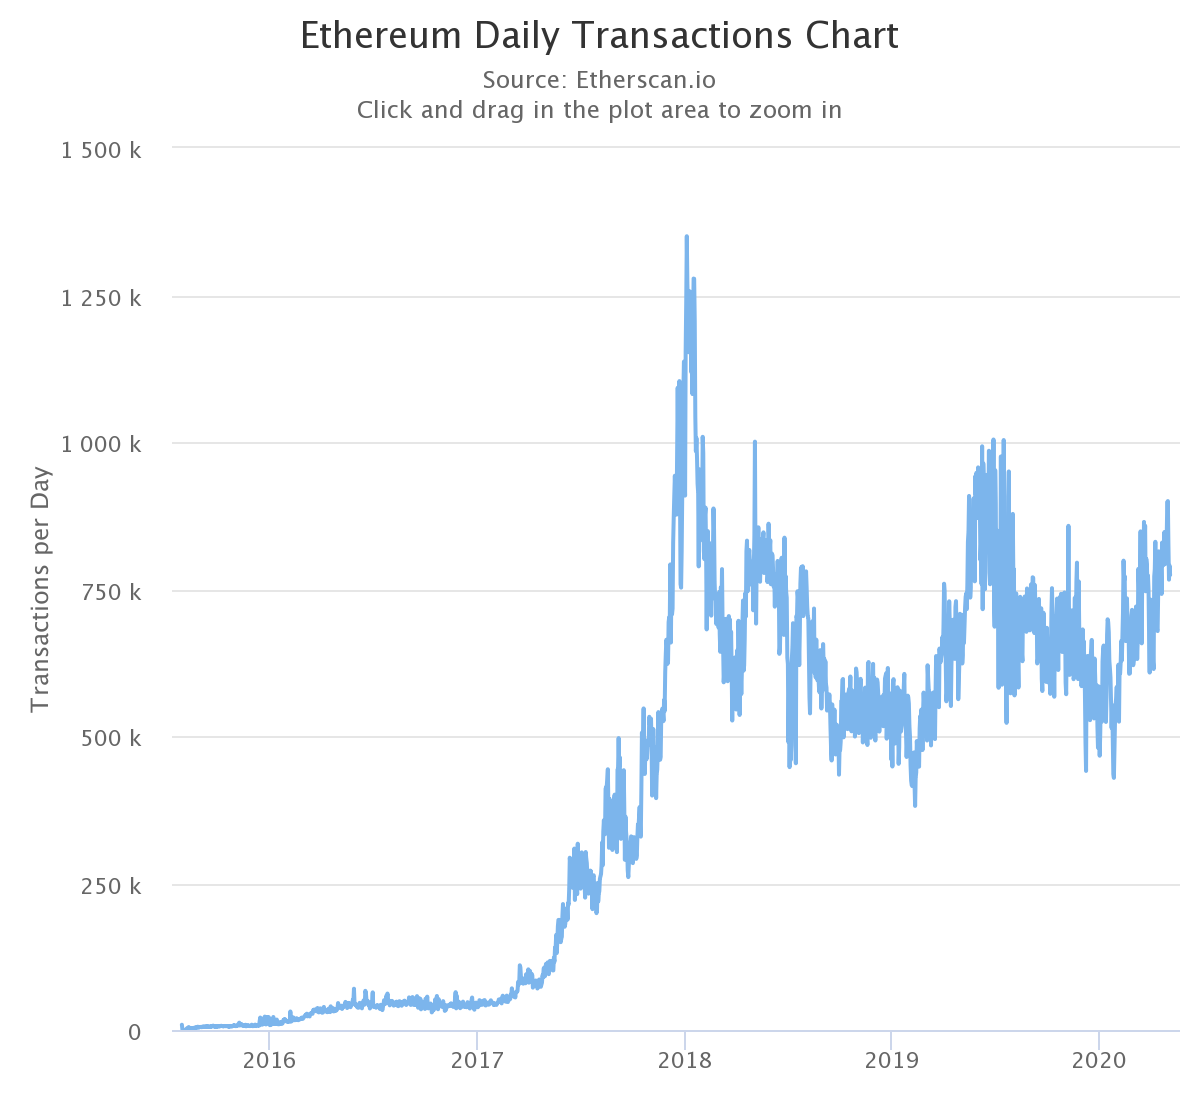
\includegraphics[scale=0.235]{daily_txs_chart.png}
            \caption{}\label{fig:daily_txs_chart}
        \end{figure}
    \end{frame}

    \begin{frame}{Addresses}
        \begin{block}{}
            In Ethereum and Solidity, an address is a 20 byte (160 bits or 40 hex characters) alphanumeric string.
            It corresponds to the last 20 bytes of the Keccak-256 hash of the public key.
        \end{block}

        \begin{figure}
            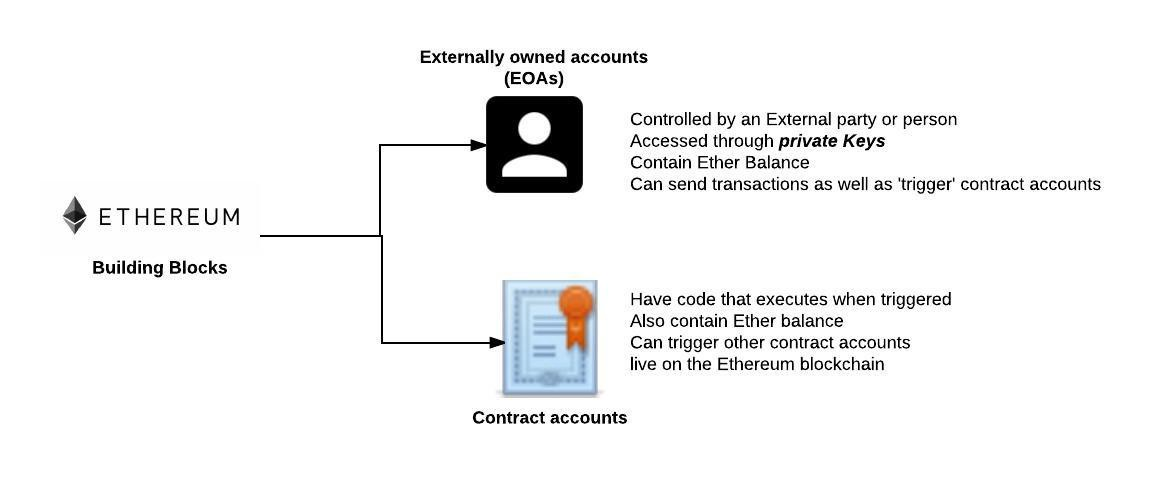
\includegraphics[width=\textwidth]{types_of_addresses.jpeg}
            \caption{Source: \href{https://hackernoon.com/heres-how-i-built-a-private-blockchain-network-and-you-can-too-62ca7db556c0}{Abhishek Chakravarty, Hackernoon.com}}\label{fig:types_of_addresses}
        \end{figure}

    \end{frame}

    \begin{frame}{Transactions}
        \begin{block}{}
            While transactions are used for different purposes, the transaction structure is the same.
            The amount of fund is expressed in wei (1 ether = $10^{18}$ weis).
            Contracts can receive transfers just like externally controlled accounts, but they can also receive more complicated transactions that actually run parts of their code and update their state.
        \end{block}

        \vskip 0.5cm

        \begin{block}{Types}
            \begin{itemize}
                \item \textbf{Fund Transfer Between EOA} used when an EOA is transferring fund to another EOA\@.
                \item \textbf{Deploy a Contract on Ethereum Network} used to deploy a compiled contract
                \item \textbf{Execute a Function on a Deployed Contract}
            \end{itemize}
        \end{block}
    \end{frame}

    \section{Methods}\label{sec:methods}

    \begin{frame}{Clustering coefficients}
        \begin{block}{}
            Undirected graph $G = (V,E)$ without self loops and multiple edges.
        \end{block}

        \vskip 0.5cm

        \begin{block}{Transitivity}
            The fraction of all possible triangles (closed triplets) present in G. Possible triangles are identified by the number of “triads” (two edges with a shared vertex, open and closed triplets): $3\cfrac{|\delta(G)|}{|\tau(G)|}$
        \end{block}

        \begin{block}{Global clustering coefficient}
            The sum of fractions of number of triangles over number of open or closed triples passing on each vertex with degree greater than 2:
            $\cfrac{1}{|V_2|} \sum_{i \in V_2}\cfrac{|\delta(v_i)|}{|\tau(v_i)|}$
        \end{block}
    \end{frame}

    \begin{frame}

        \begin{block}{Local clustering coefficient}
            Quantifies how close the neighbours of a vertex in a graph are to being a clique (complete graph): $\cfrac{2|\{e_{jk} : v_j, v_k \in N_i, e_{jk} \in E\}|}{|N_i|(|N_i| - 1)}$
        \end{block}

        \begin{block}{}
            Where $E$ is the set of edges and $V$ the set of vertices. $N_i$ is the set of neighbors of the node $v_i \in V$. $V_2$ is the set $\{v_i \in V: |N_i| \geq 2$\}.
            The set of triangles is expressed with the function $\delta(x)$ and the set of open and closed triplets with $\tau(x)$.
        \end{block}

    \end{frame}

    \begin{frame}{Modularity}
        \begin{block}{}
            Measure the strength of division of a network into \textbf{modules (also called groups, clusters or communities)}.
            Networks with high modularity have dense connections between the nodes within modules but sparse connections between nodes in different modules.
        \end{block}
        \begin{block}{}
            $\sum_{i=1}^{c}(e_{ii} - a_{i}^{2})$, where $e_{ij}$ is the fraction of edges in the community $i$ to community $j$ and $a_i$ is $\sum_je_{ij}$
        \end{block}

        \begin{block}{}
            Fraction of edges that fall within communities, minus the expected value of the same quantity if edges fall at random without regard for the community structure, which is the total degree of the cluster.
        \end{block}
    \end{frame}

    \begin{frame}{Community Detection}
        \begin{block}{Two different concepts}
            \begin{itemize}
                \item Clustering
                \item Partitioning
            \end{itemize}
        \end{block}
        \begin{block}{Clustering methods}
            \begin{itemize}
                \item \textbf{Label Propagation}
                \item Louvain Method
                \item Minimum Cut Three
                \item Dynamic Clustering
            \end{itemize}
        \end{block}

    \end{frame}

    \section{Results}\label{sec:results}

    \begin{frame}{Results}
        \begin{block}{Clustering Coefficients}
            The measured global coefficient is between 0.02 and 0.03 and almost the 95\% of vertices have a local cluster coefficient equal to 0.
            That may depends also on the way the data is collected and distributed temporally and spatially in the Blockchain the network seems to be very sparse.
        \end{block}

        \vskip 0.75cm

        \begin{block}{Modularity}
            The graph could be divided in many connected components, in a network of more than 10 thousands vertices there are almost 1 thousands groups.
            The biggest connected component includes almost half of the vertices and the modularity of its clustering in almost 700 communities is near 0 (from -0.5 to 1).
        \end{block}
    \end{frame}

    \begin{frame}{}
        \begin{block}{Community detection}
            \begin{figure}
                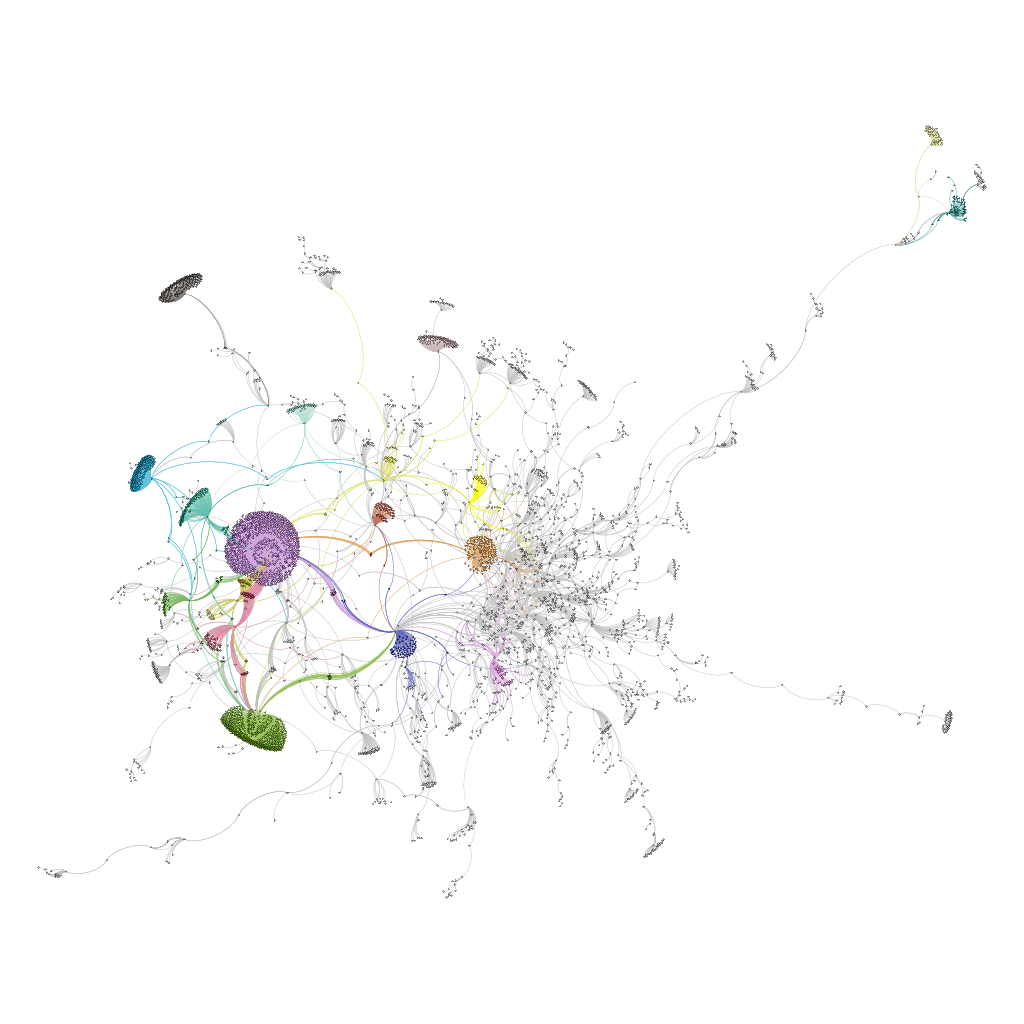
\includegraphics[scale=0.2]{gephi_1.png}
                \caption{The greatest connected component rendered on Gephi}\label{fig:gephi_1}
            \end{figure}
        \end{block}
    \end{frame}

    \begin{frame}{Further works}
        \begin{block}{Deanonymize the network}
            Scraping from the web more features to associate to the addresses, (forums, datasets etc..)
        \end{block}

        \vskip 1cm

        \begin{block}{Cluster users}
            Apply Machine Learning/Data Mining techniques to cluster addresses based on activity (Miners, ICO, etc..) in addition to the study of the topology structure
        \end{block}
    \end{frame}

    \section{References}\label{sec:references}

    \begin{frame}{References}
        \begin{itemize}
            \item \href{https://medium.com/@kctheservant/transactions-in-ethereum-e85a73068f74}{Transactions in Ethereum, KC Tam, Medium}
            \item \href{https://www.sci.unich.it/~francesc/teaching/network/transitivity.html}{Transitivity, Massimo Franceschet, University of Udine}
            \item \href{http://algo2.iti.kit.edu/schulz/gpgc_vorlesung/graphpartitioning_lecture.pdf}{Graph Partitioning and Graph Clustering in Theory and Practice, Christian Schulz, Institute for Theoretical Informatics Karlsruhe Institute of Technology}
        \end{itemize}
    \end{frame}

\end{document}
